\documentclass[aspectratio=169, 10pt]{beamer}

% --- Theme and Visual Setup ---
\usetheme{metropolis}
\metroset{
  progressbar=frametitle,
  block=fill,
  titleformat frame=regular
}

% --- Packages ---
\usepackage{amsmath}
\usepackage{graphicx}
\usepackage{booktabs}
\usepackage{tabularx}
\usepackage{makecell}
\usepackage{xcolor}
\usepackage{subcaption}
\usepackage{colortbl}
\usepackage{listings}

% --- Custom Colors & Visual Styling ---
\definecolor{darkblue}{RGB}{20, 40, 80}
\definecolor{tealaccent}{RGB}{0, 128, 128}
\definecolor{lightgraybg}{RGB}{245, 247, 250}
\definecolor{codegray}{rgb}{0.5,0.5,0.5}

\setbeamercolor{frametitle}{fg=white, bg=darkblue}
\setbeamercolor{progress bar}{fg=tealaccent, bg=gray!30}
\setbeamercolor{alerted text}{fg=tealaccent}
\setbeamercolor{block title}{fg=white, bg=darkblue}
\setbeamercolor{block body}{fg=black, bg=lightgraybg}

\lstdefinelanguage{json}{
    basicstyle=\ttfamily\tiny,
    showstringspaces=false,
    breaklines=true,
    string=[s]{"}{"},
    stringstyle=\color{blue!80!black},
    comment=[l]{//},
    morecomment=[s]{/*}{*/},
    commentstyle=\color{codegray},
    literate=
     *{0}{{{\color{black}0}}}{1}
      {1}{{{\color{black}1}}}{1}
      {2}{{{\color{black}2}}}{1}
      {3}{{{\color{black}3}}}{1}
      {4}{{{\color{black}4}}}{1}
      {5}{{{\color{black}5}}}{1}
      {6}{{{\color{black}6}}}{1}
      {7}{{{\color{black}7}}}{1}
      {8}{{{\color{black}8}}}{1}
      {9}{{{\color{black}9}}}{1}
}

% --- Metadata ---
\title[ReXGroundingCT 3D Data Profiling]{ReXGroundingCT 3D Data Profiling, Spatial Priors \& Prompt Syntax}
\subtitle{MICCAI 2026 Challenge Benchmark Investigation}
\author{Joaquín De Ferrari}
\date{July 28, 2026}

\begin{document}

% ==============================================================================
% SLIDE 1: Title
% ==============================================================================
\begin{frame}
    \titlepage
    \note{
        Welcome everyone to our Phase 1 technical report presentation on ReXGroundingCT.
        In this talk, we present our systematic data profiling investigation across 3,078 physical CT scans and 8,650 radiology report prompts, covering split annotation disparity, free-text NLP syntax shift, canonical 3D RAS spatial priors, HU radiodensity windowing, and 3D component morphology.
    }
\end{frame}

% ==============================================================================
% SLIDE 2: Dataset Hierarchy
% ==============================================================================
\begin{frame}{Dataset Indexing Hierarchy}
    \vspace{-0.5em}
    \begin{block}{Tier 1: Physical NIfTI Scans (3,078 Volumes)}
        \footnotesize 2,578 Train / 200 Val / 300 Test physical scan acquisition sessions.
    \end{block}
    
    \vspace{-0.3em}
    \centering \tiny \color{tealaccent} $\downarrow$ Multi-kernel series indexing (\texttt{\_1.nii.gz}, \texttt{\_2.nii.gz}) \color{black}
    \vspace{-0.3em}
    
    \begin{block}{Tier 2: Dataset Record Entries (3,192 Records)}
        \footnotesize 2,992 Train / 200 Val indexed entries in \texttt{dataset.json} (with raw reports).
    \end{block}
    
    \vspace{-0.3em}
    \centering \tiny \color{tealaccent} $\downarrow$ GPT-4 parses raw reports into discrete finding text queries \color{black}
    \vspace{-0.3em}
    
    \begin{block}{Tier 3: Report Prompts (8,650 Free-Text Queries)}
        \footnotesize 8,650 radiology sentence prompts (81.4\% unique verbatim text).
    \end{block}
    
    \vspace{-0.3em}
    \centering \tiny \color{tealaccent} $\downarrow$ Radiologists segment 3D voxel masks paired to each text query \color{black}
    \vspace{-0.3em}
    
    \begin{block}{Tier 4: Target Finding Masks (8,650 3D Masks)}
        \footnotesize 7,687 Train (Entity protocol $\le 3$) / 381 Val (Exhaustive) / 582 Test 3D segmentation masks.
    \end{block}

    \note{
        To understand the ReXGroundingCT dataset, we first look at its 4-tier indexing hierarchy.

        At Tier 1, the benchmark consists of 3,078 physical CT scan acquisition sessions derived from the CT-RATE repository, split into 2,578 training, 200 validation, and 300 test volumes.

        Moving to Tier 2, there are 3,192 indexed entries in dataset.json. This number is slightly higher than physical scans because some patient examinations were reconstructed under multiple scanner kernels, such as thin and thick slice series.

        At Tier 3, GPT-4 parsed the raw clinical radiology reports to extract 8,650 discrete finding prompts. Over 81 percent of these prompts are unique verbatim sentences. The remaining 19 percent are exact duplicate phrases, which occur because radiologists use standardized clinical report templates for common findings, and because multi-kernel series from the same scan inherit the exact same report text.

        Finally, at Tier 4, human radiologists manually annotated 8,650 3D segmentation masks paired 1-to-1 with each text prompt. In the training split, annotators capped representative lesions at 3 per finding under the Entity Protocol, whereas the validation split features unconstrained exhaustive annotations.
    }
\end{frame}

% ==============================================================================
% SLIDE 2b: Dataset Record Entry Anatomy (dataset.json)
% ==============================================================================
\begin{frame}[fragile]{Dataset Record Entry Anatomy (\texttt{dataset.json})}
    \begin{columns}[c]
        \begin{column}{0.58\textwidth}
\begin{lstlisting}[language=json,basicstyle=\ttfamily\scriptsize]
{
  "name": "train_1935_a_1.nii.gz",
  "findings": {
    "0": "Peribronchial thickening in both lungs",
    "1": "Mosaic attenuation in both lungs",
    "2": "Paraseptal emphysema in apices",
    "3": "Pulmonary nodules in both lungs"
  },
  "entity_counts": {
    "0": 2, "1": 3, "2": 3, "3": 3
  },
  "shape": [512, 512, 264],
  "pixels": {
    "0": 101934, "1": 315619, "2": 7065, "3": 772
  },
  "categories": {
    "0": "1a", "1": "1f", "2": "1c", "3": "2d"
  }
}
\end{lstlisting}
        \end{column}
        \begin{column}{0.40\textwidth}
            \begin{block}{Indexed Record Schema}
                \scriptsize
                \begin{itemize}
                    \item \textbf{\texttt{"name"}}: NIfTI file ID (\texttt{\_1} = series 1).
                    \item \textbf{\texttt{"findings"}}: Report text queries.
                    \item \textbf{\texttt{"entity\_counts"}}: Instance counts ($\le 3$).
                    \item \textbf{\texttt{"shape"}}: 3D grid $[512, 512, 264]$.
                    \item \textbf{\texttt{"pixels"}}: Total voxel count per mask.
                    \item \textbf{\texttt{"categories"}}: Category codes.
                \end{itemize}
            \end{block}
        \end{column}
    \end{columns}

    \note{
        On this slide, we see a concrete record entry from dataset.json for scan train\_1935\_a\_1.

        Each entry indexes:
        First, the physical NIfTI filename. Note the underscore-one suffix, indicating reconstruction series 1 for this patient.
        Second, the findings dictionary, containing the exact text prompts extracted from the radiology report.
        Third, the entity counts, showing how many 3D instances were annotated for each finding—for instance, 3 nodules or 2 areas of bronchial thickening.
        Fourth, the 3D grid shape and total voxel count for each ground-truth binary mask.
        And finally, the category mapping, which assigns each text query to one of the 14 benchmark pathology codes.
    }
\end{frame}

% ==============================================================================
% SLIDE 3: Table 1 - Dataset Split Overview & Disparity
% ==============================================================================
\begin{frame}{Dataset Split Overview \& Disparity}
    \centering
    \small
    \begin{tabular}{lcccccc}
        \toprule
        \textbf{Split} & \makecell{\textbf{Records /}\\\textbf{Physical Scans}} & \textbf{Findings} & \makecell{\textbf{Findings}\\\textbf{/ Record}} & \makecell{\textbf{Mean Inst}\\\textbf{/ Finding}} & \textbf{Std Inst} & \textbf{Max Inst} \\
        \midrule
        \textbf{Train} & 2,992 (2,578) & 7,687 & 2.57 & 1.948 & $\pm 0.962$ & 11 \\
        \rowcolor{darkblue!10}
        \textbf{Val}   & 200 (200)     & 381   & 1.91 & \textbf{3.714} & $\pm 4.441$ & \textbf{36} \\
        \textbf{Test}  & 300 (300)     & 582   & 1.94 & -- & -- & -- \\
        \bottomrule
    \end{tabular}

    \vspace{1.0em}
    \begin{columns}[c]
        \begin{column}{0.95\textwidth}
            \begin{itemize}
                \item \textbf{Train Protocol:} Entity Protocol capping annotated instances ($\le 3$ per finding query).
                \item \textbf{Val Protocol:} Exhaustive annotation of all visible instances ($1.91\times$ quantitative disparity).
                \item \textbf{Test Split Note:} Test instance statistics are withheld pending official challenge evaluation.
            \end{itemize}
        \end{column}
    \end{columns}

    \note{
        In this summary, we present the primary dataset split composition and highlight the fundamental annotation disparity between training and validation sets.

        The dataset comprises 2,992 training records, 200 validation records, and 300 test records. Across all splits, scans average around 1.9 to 2.5 finding queries per scan.

        However, look closely at the mean instances per finding column: in the Training set, findings average 1.95 instances, with a maximum of 11 connected components (which occurs when complex annotated masks fragment in 3D space). This reflects the Entity Protocol, which capped human annotations at at most 3 entities per finding query.

        In contrast, the Validation set features unconstrained exhaustive annotations, averaging 3.71 instances per finding and reaching up to 36 instances in multi-focal cases. This produces a global 1.91x quantitative annotation disparity between splits.

        Note that Test split instance statistics are marked with dashes because test ground-truth masks are withheld by challenge organizers pending official leaderboard evaluation.
    }
\end{frame}

% ==============================================================================
% SLIDE 4: Table 2 - 14-Category Breakdown
% ==============================================================================
\begin{frame}{14-Category Breakdown \& Disparity Ratios}
    \centering
    \tiny
    \setlength{\tabcolsep}{6pt}
    \begin{tabular}{clcccccc}
        \toprule
        \textbf{Code} & \textbf{Category Name} & \textbf{Type} & \textbf{Train Prev (\%)} & \textbf{Val Prev (\%)} & \textbf{Train Mean Inst.} & \textbf{Val Mean Inst.} & \textbf{Disparity Ratio} \\
        \midrule
        \texttt{1a} & Bronchial wall thickening & Non-Focal & 7.09 & 1.50 & 2.05 & 4.00 & 1.95x \\
        \texttt{1b} & Bronchiectasis           & Non-Focal & 8.26 & 4.50 & 2.10 & 3.27 & 1.56x \\
        \texttt{1c} & Emphysema                & Non-Focal & 13.97 & 7.50 & 2.39 & 2.82 & 1.18x \\
        \texttt{1d} & Septal thickening        & Non-Focal & 6.15 & 3.00 & 2.22 & 5.50 & 2.48x \\
        \texttt{1e} & Micronodules             & Non-Focal & 7.99 & 5.50 & 2.21 & 5.18 & 2.35x \\
        \texttt{1f} & Other non-focal          & Non-Focal & 4.75 & 2.00 & 2.08 & 2.75 & 1.32x \\
        \midrule
        \texttt{2a} & Linear opacities         & Focal & 26.77 & 31.50 & 1.71 & 2.25 & 1.31x \\
        \texttt{2b} & Atelectasis / consolid.  & Focal & 30.45 & 20.00 & 1.78 & 2.78 & 1.56x \\
        \rowcolor{blue!10}
        \texttt{2c} & Ground-glass opacity     & Focal & 37.73 & 26.50 & 2.23 & \textbf{7.13} & \textbf{3.20x} \\
        \texttt{2d} & Pulmonary nodules/masses & Focal & \textbf{43.62} & \textbf{59.50} & 1.83 & 3.53 & 1.93x \\
        \texttt{2e} & Pleural effusion/thick.  & Focal & 6.08 & 5.50 & 1.43 & 2.00 & 1.40x \\
        \texttt{2f} & Honeycombing             & Focal & 0.50 & 0.00 & 2.06 & -- & -- \\
        \texttt{2g} & Pneumothorax             & Focal & 1.20 & 2.50 & 1.19 & 1.40 & 1.17x \\
        \texttt{2h} & Other focal              & Focal & 0.97 & 1.50 & 1.28 & 2.00 & 1.57x \\
        \bottomrule
    \end{tabular}

    \note{
        This table provides the fine-grained 14-category breakdown across non-focal pathologies (types 1a through 1f) and focal pathologies (types 2a through 2h).

        First, notice scan prevalence: Pulmonary nodules and masses (category 2d) is the most prevalent pathology in the dataset, appearing in 43.6 percent of training scans and nearly 60 percent of validation scans. Ground-glass opacity (category 2c) and Atelectasis (category 2b) are also highly prevalent focal findings.

        Second, observe the annotation disparity ratio column. Ground-glass opacity exhibits the highest disparity in the entire benchmark—a 3.20-fold jump from 2.23 instances per query in training to 7.13 instances in exhaustive validation. Septal thickening and Micronodules also show over 2.3-fold instance jumps.

        Finally, Honeycombing (category 2f) is a rare finding in the dataset with 0.5 percent training prevalence and 0 validation cases, which we take into account during cross-validation modeling.
    }
\end{frame}

% ==============================================================================
% SLIDE 5: Figure 1 - Category Proportions & Findings per Scan
% ==============================================================================
\begin{frame}{Category Proportions \& Findings per Scan}
    \begin{columns}[c]
        \begin{column}{0.5\textwidth}
            \centering
            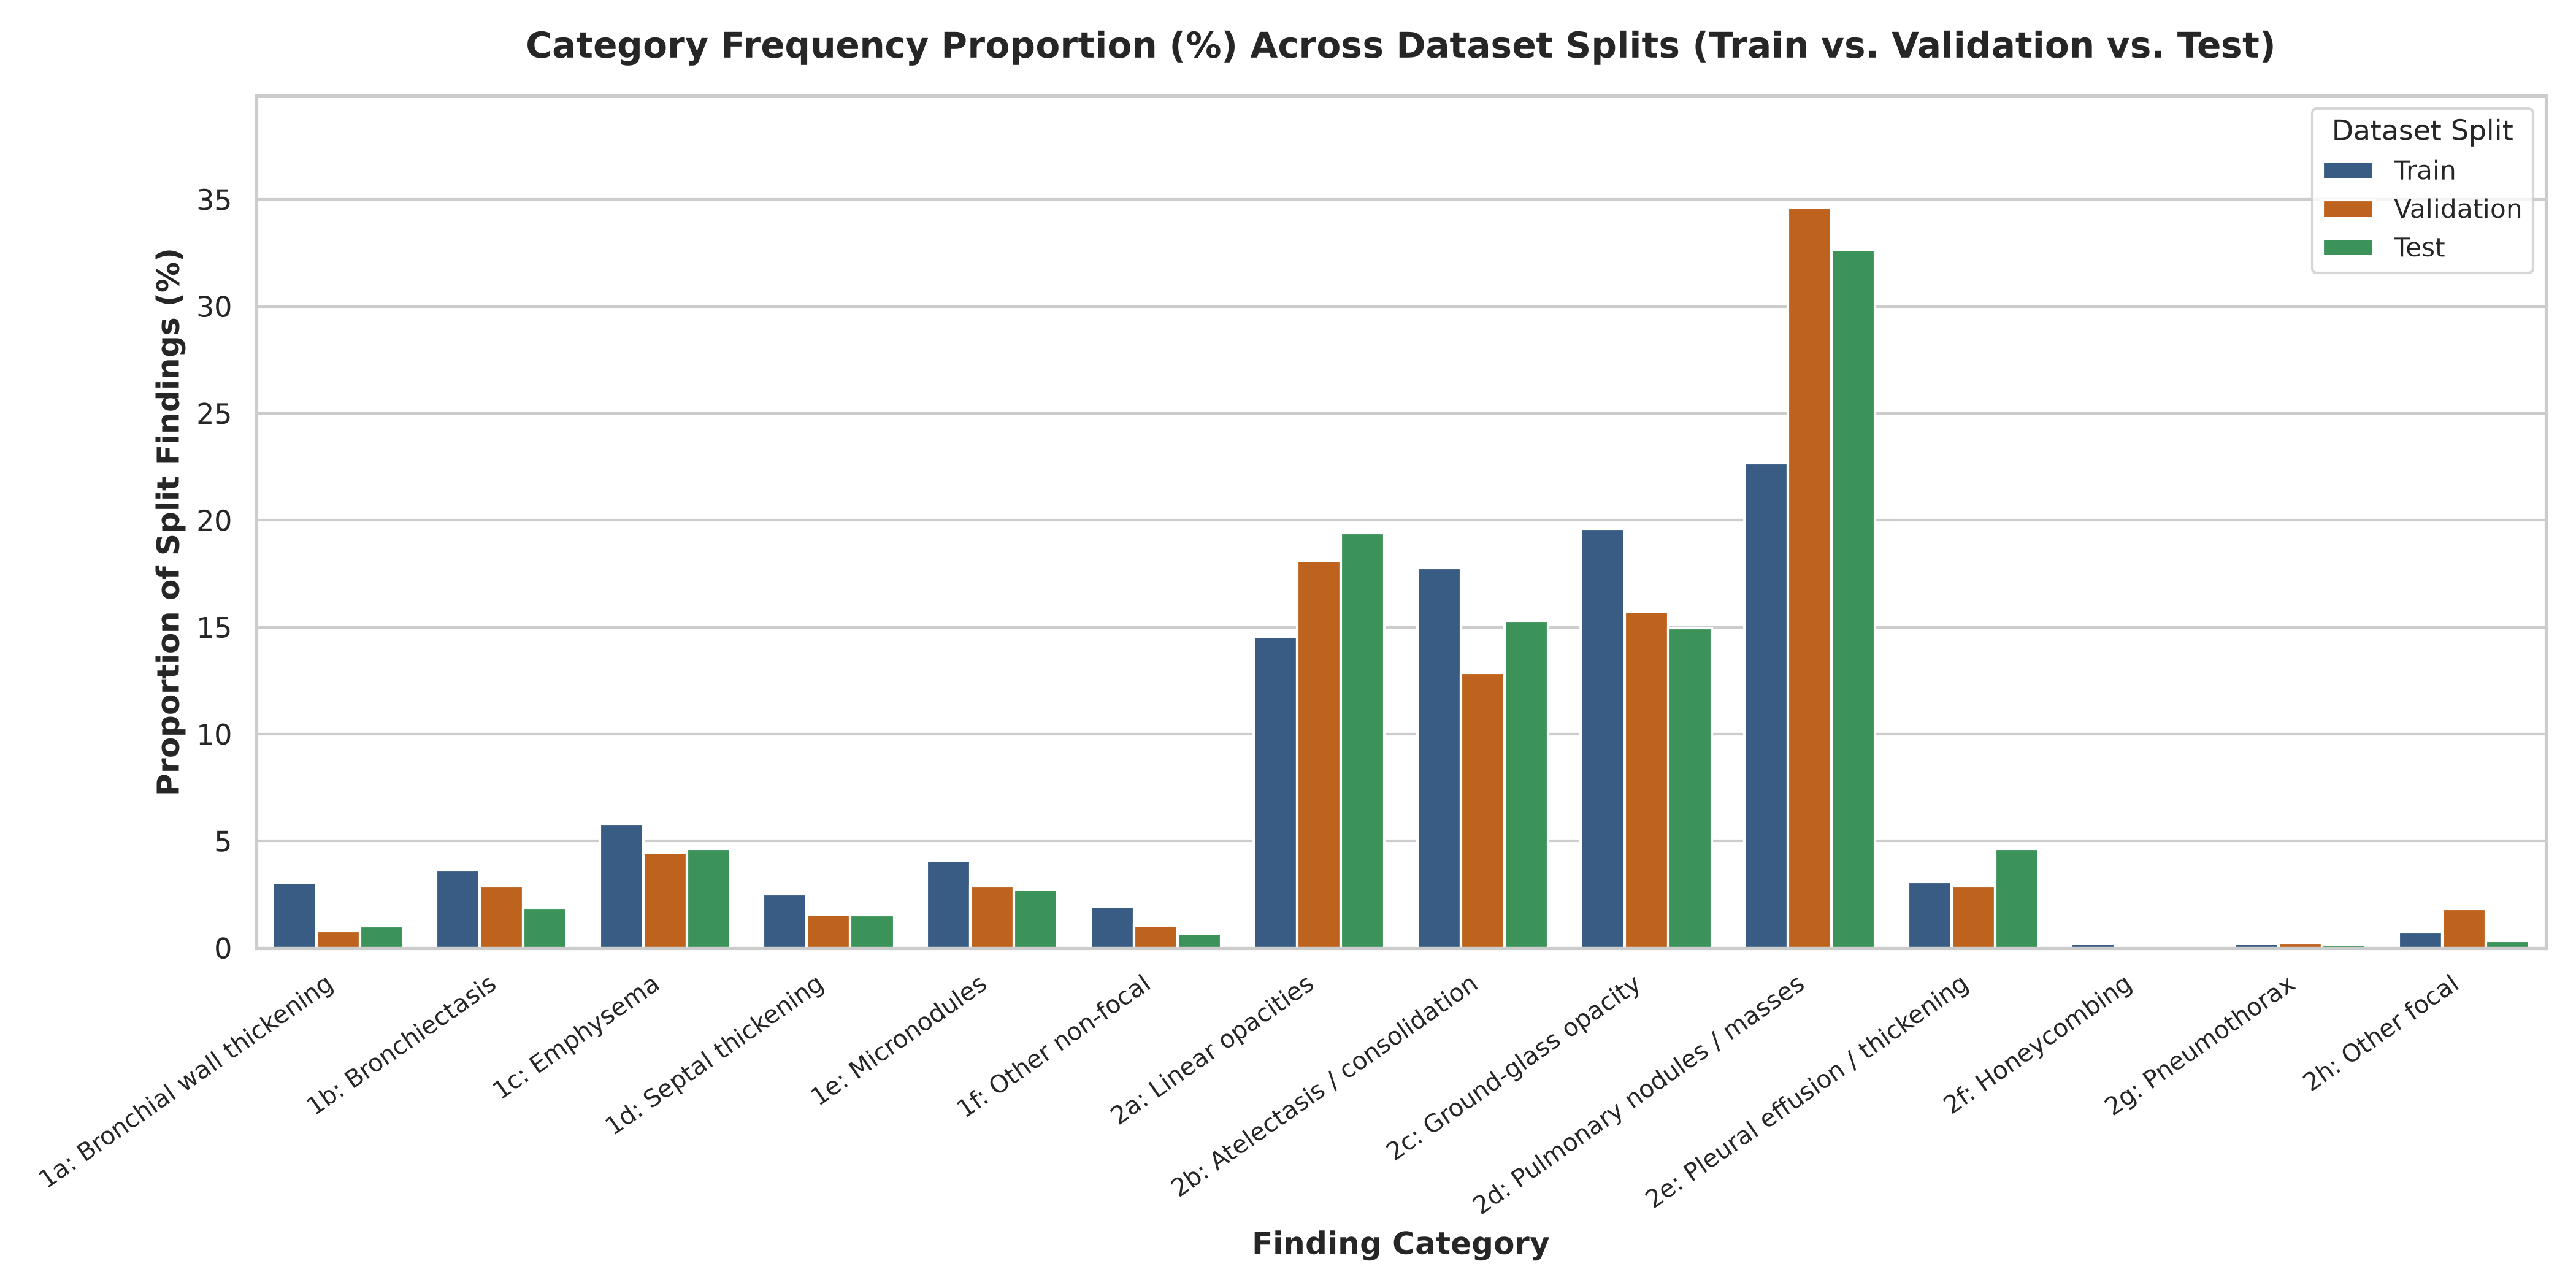
\includegraphics[width=\textwidth, height=0.68\textheight, keepaspectratio]{fig/exp001_category_frequency_breakdown.png}            
        \end{column}
        \begin{column}{0.5\textwidth}
            \centering
            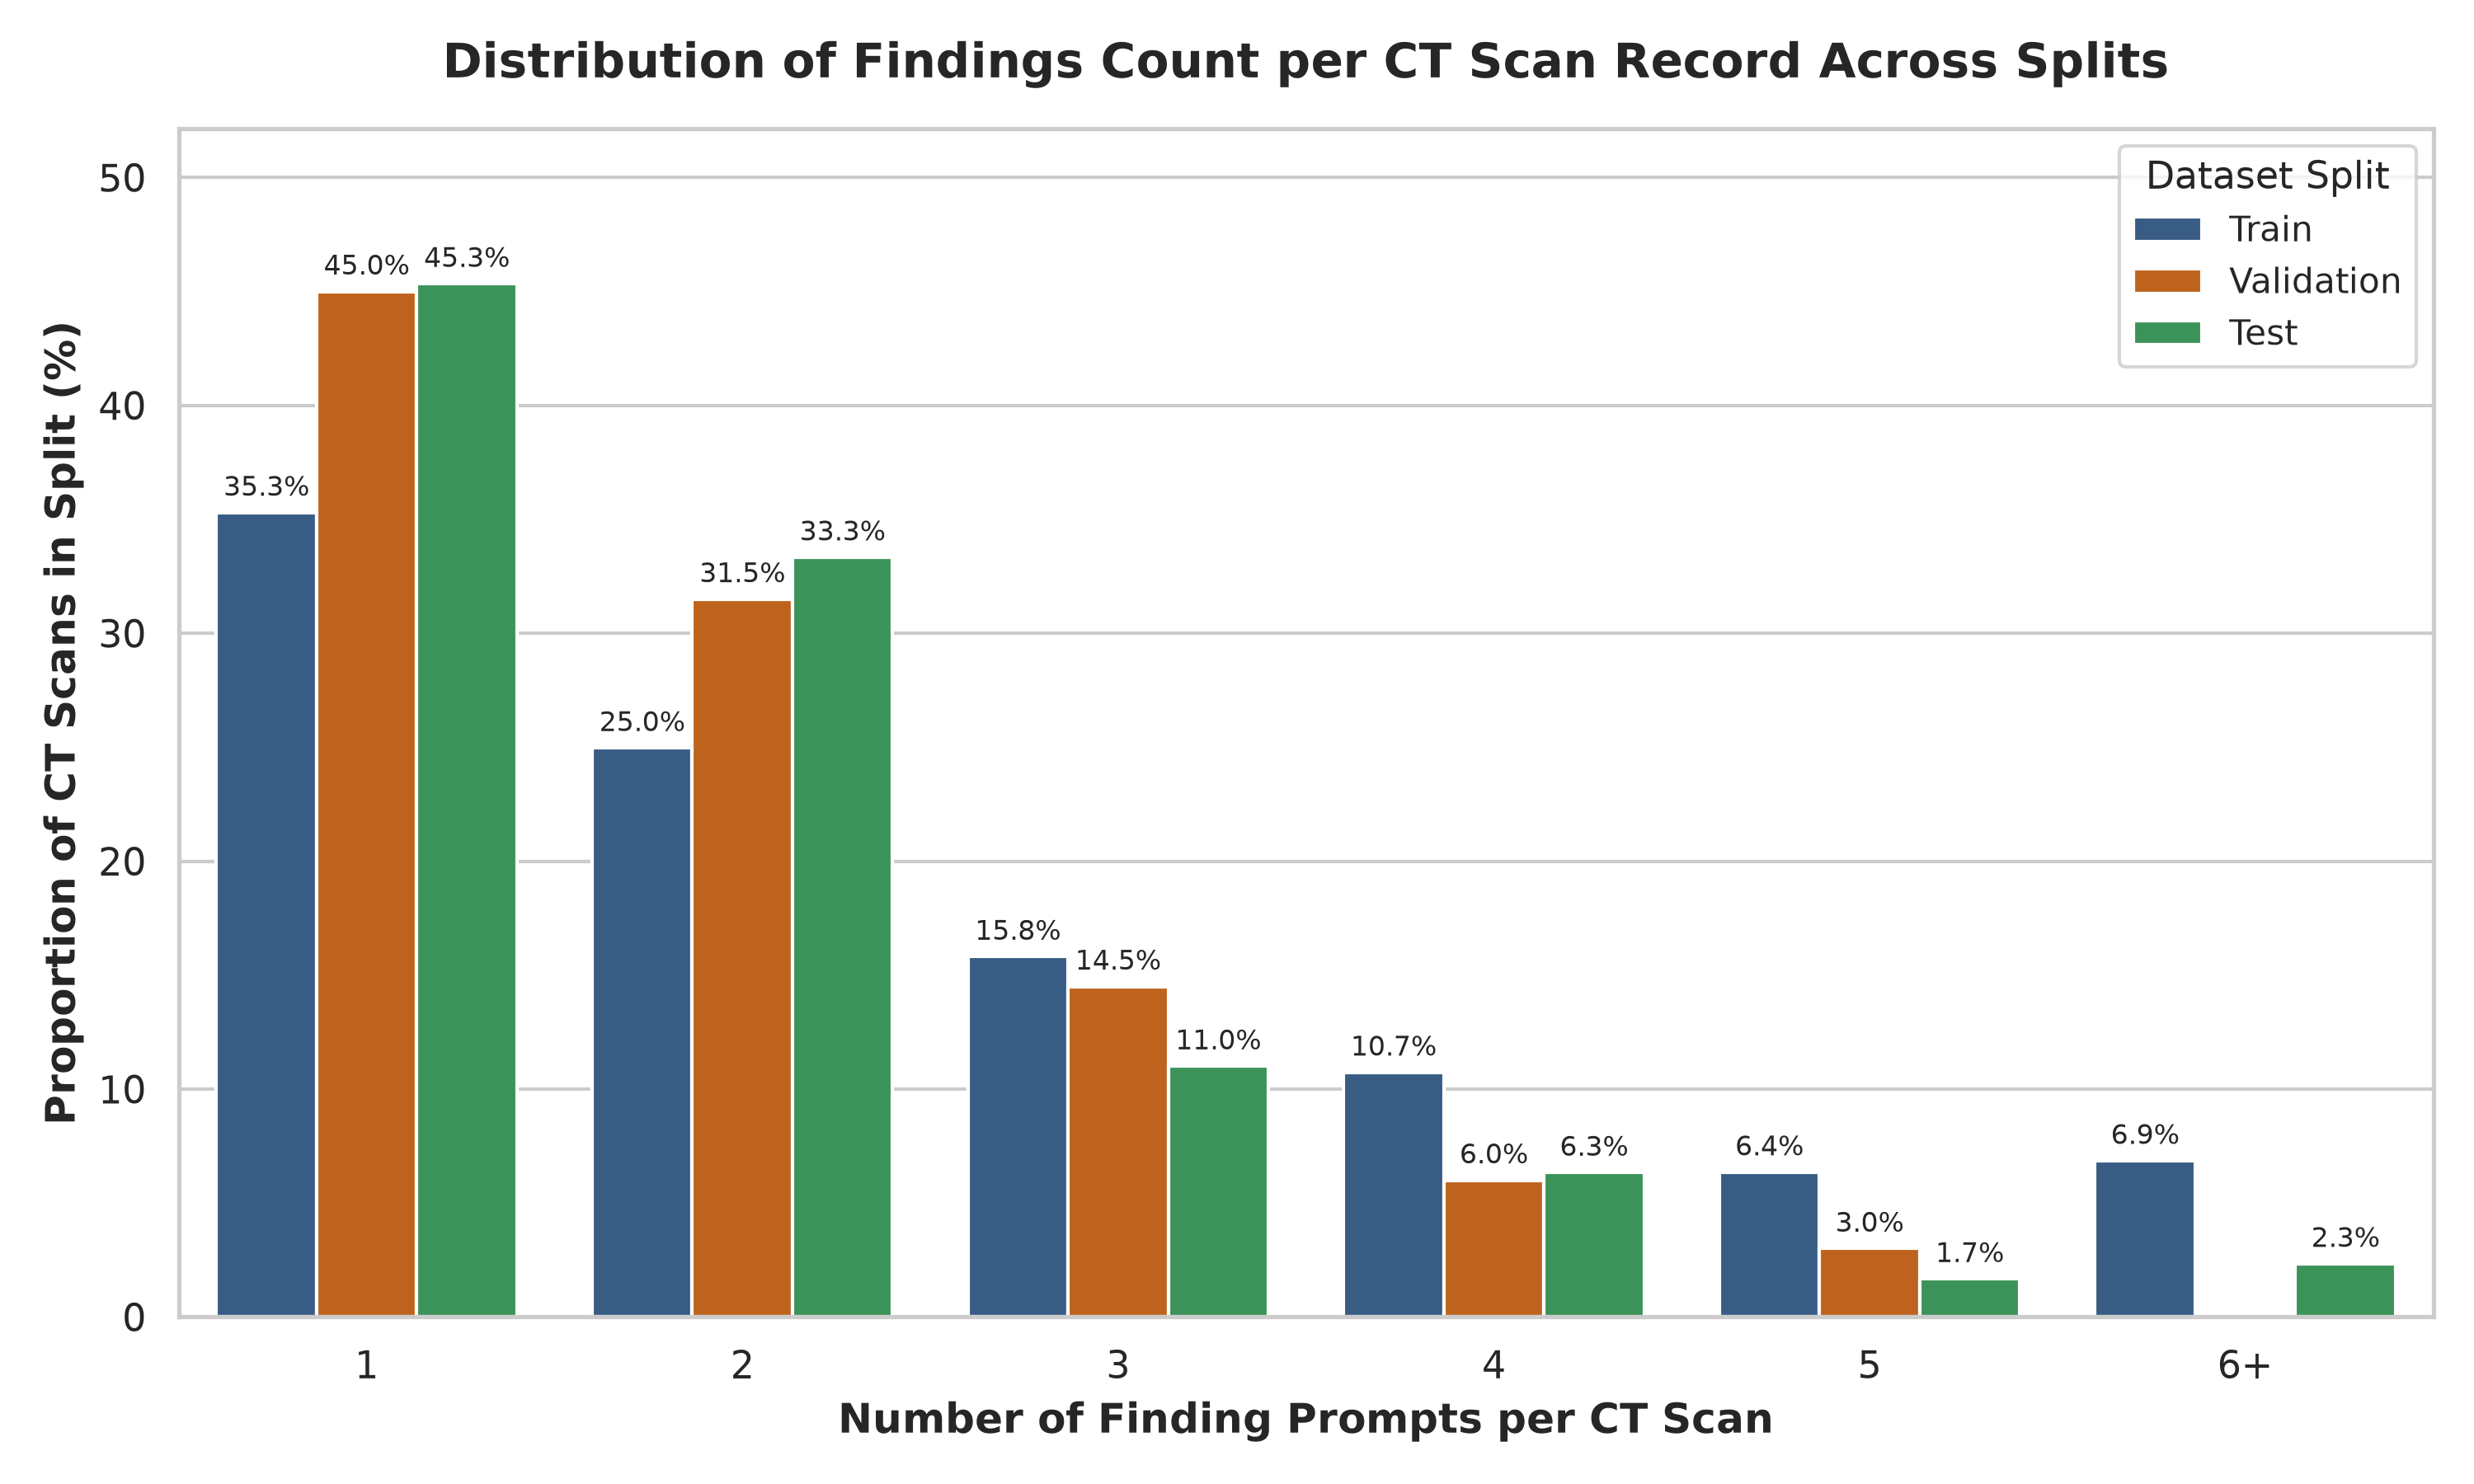
\includegraphics[width=\textwidth, height=0.68\textheight, keepaspectratio]{fig/exp001_findings_per_scan.png}        
        \end{column}
    \end{columns}

    \note{
        This slide visualizes the category proportions and findings per CT scan across the dataset splits.

        In the left plot, we see that pathology prevalence remains consistent across Training, Validation, and Test splits. Pulmonary nodules, Ground-glass opacity, and Atelectasis dominate dataset frequency, while categories like Honeycombing and Pneumothorax represent rare findings.

        In the right plot, we examine the number of finding queries per scan. CT scans in the dataset contain between 1 and 5 finding queries, averaging 2.57 findings per scan in Training and 1.91 in Validation.
    }
\end{frame}

% ==============================================================================
% SLIDE 6: Figure 2 - Connected Component Disparity
% ==============================================================================
\begin{frame}{Connected Component Instance Disparity}
    \begin{center}
        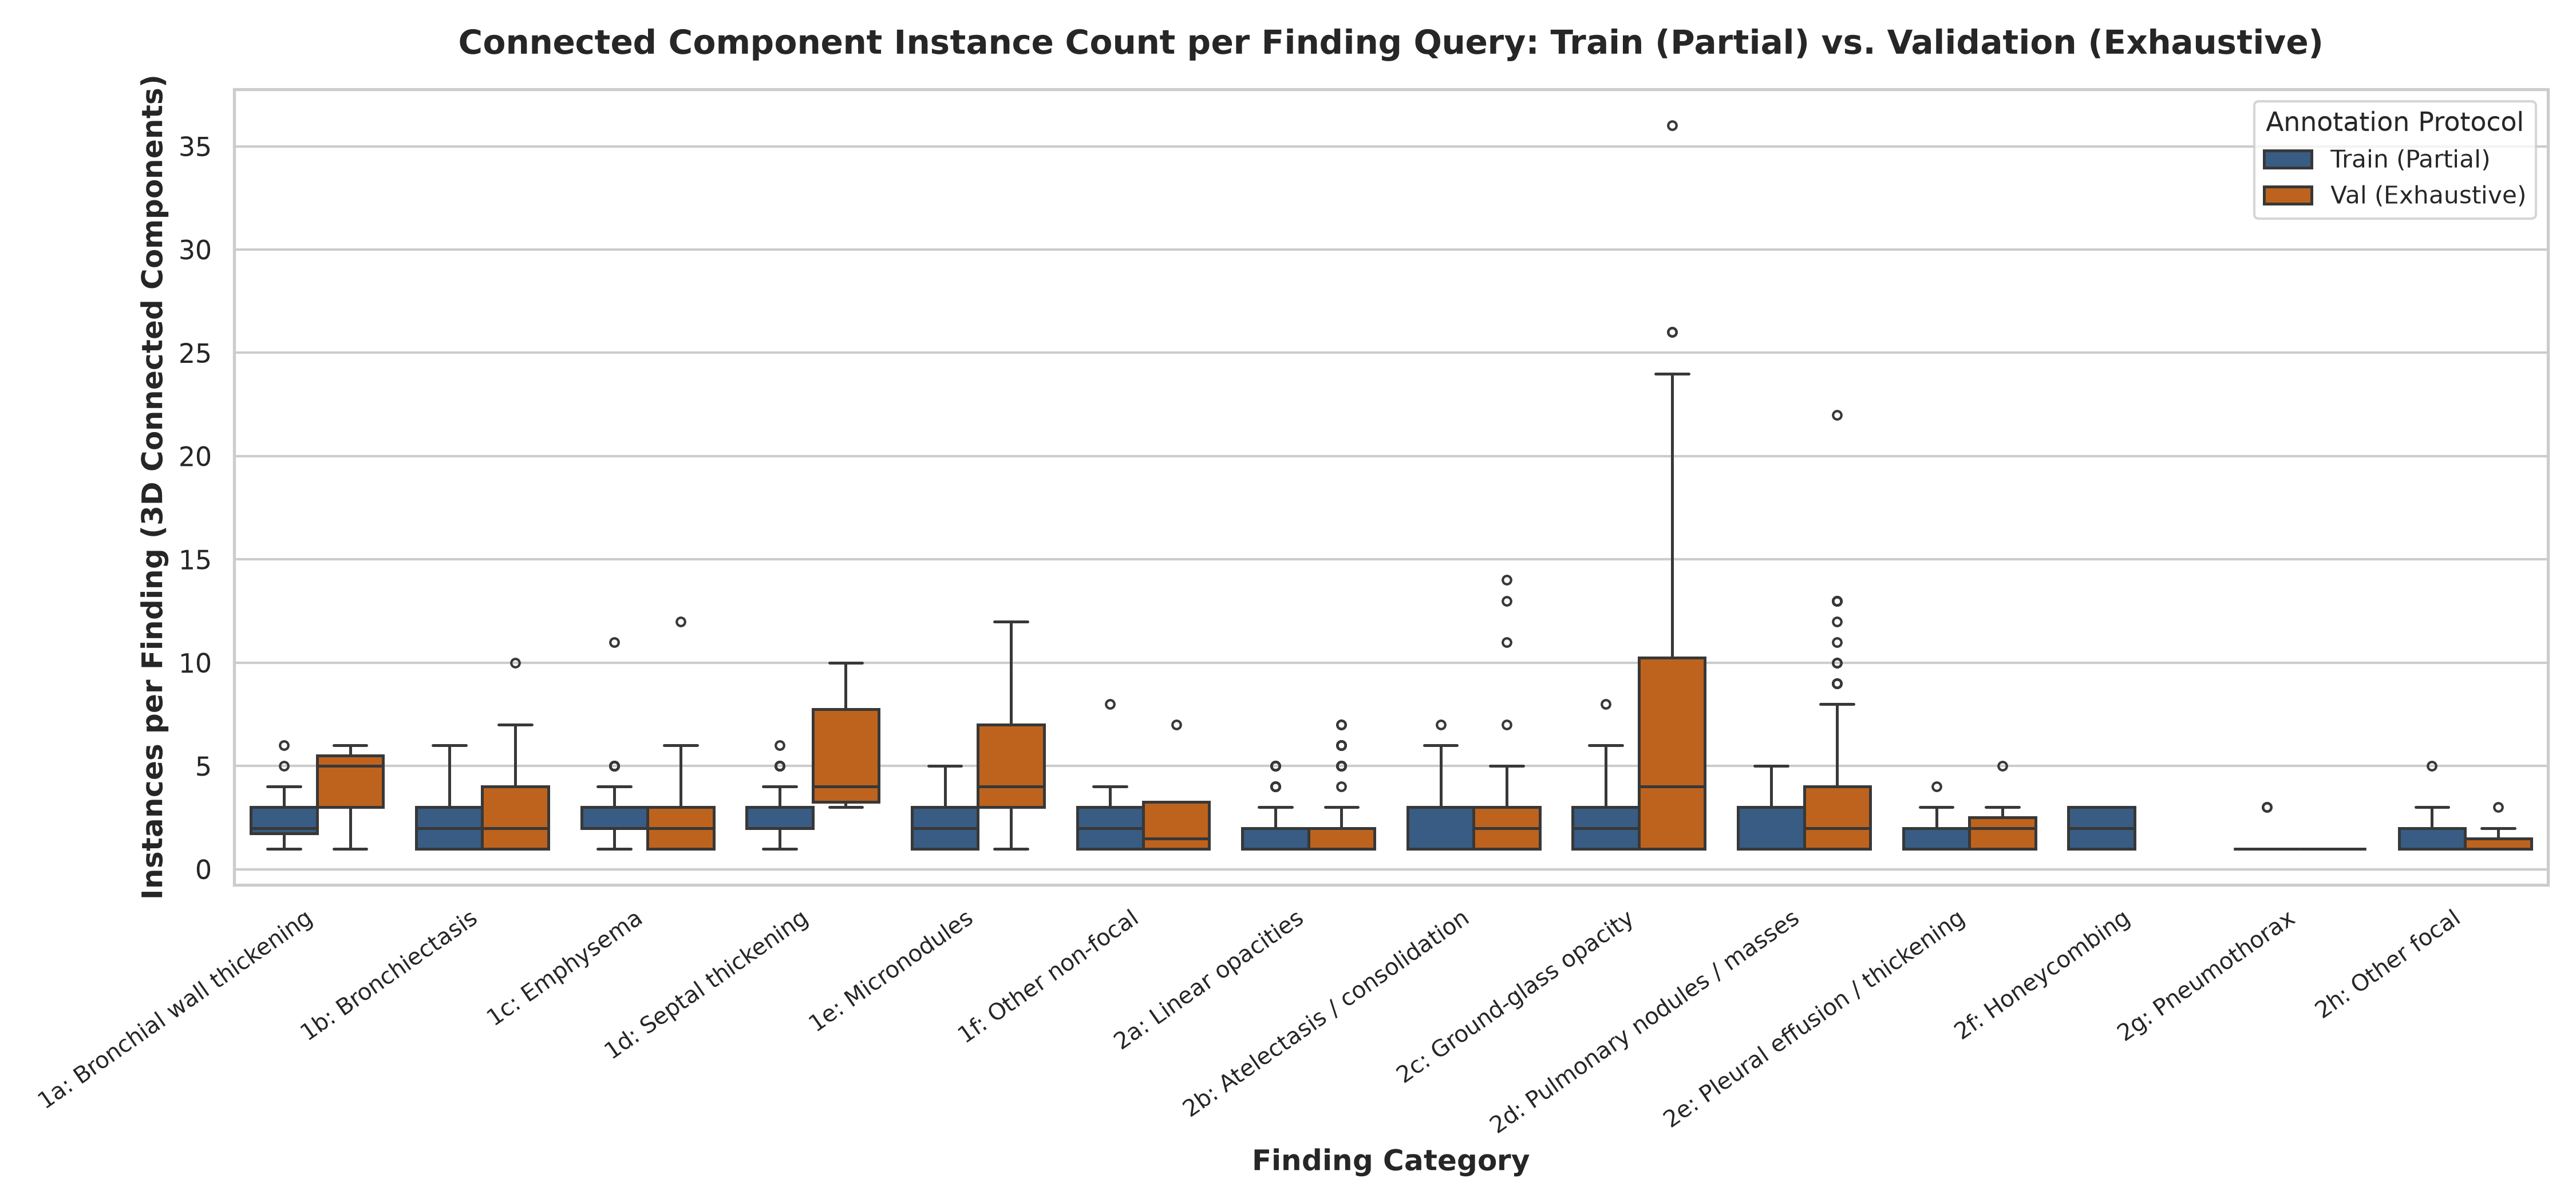
\includegraphics[width=0.88\textwidth, height=0.72\textheight, keepaspectratio]{fig/exp001_instance_count_boxplot.png}
    \end{center}

    \note{
        Here we highlight the structural boxplot comparison of connected component instance counts per finding query across all 14 categories.

        Notice the sharp contrast between the blue training boxes and orange validation boxes. In Training, instance counts are capped at at most 3 per query under the Entity Protocol. In Validation, unconstrained exhaustive annotation reveals true lesion counts, reaching up to 36 instances in Ground-glass opacity and 22 in Pulmonary nodules.
    }
\end{frame}

% ==============================================================================
% SLIDE 7: Figure 3 - Co-Occurrence Matrix
% ==============================================================================
\begin{frame}{Multi-Finding Pathology Co-Occurrence}
    \begin{center}
        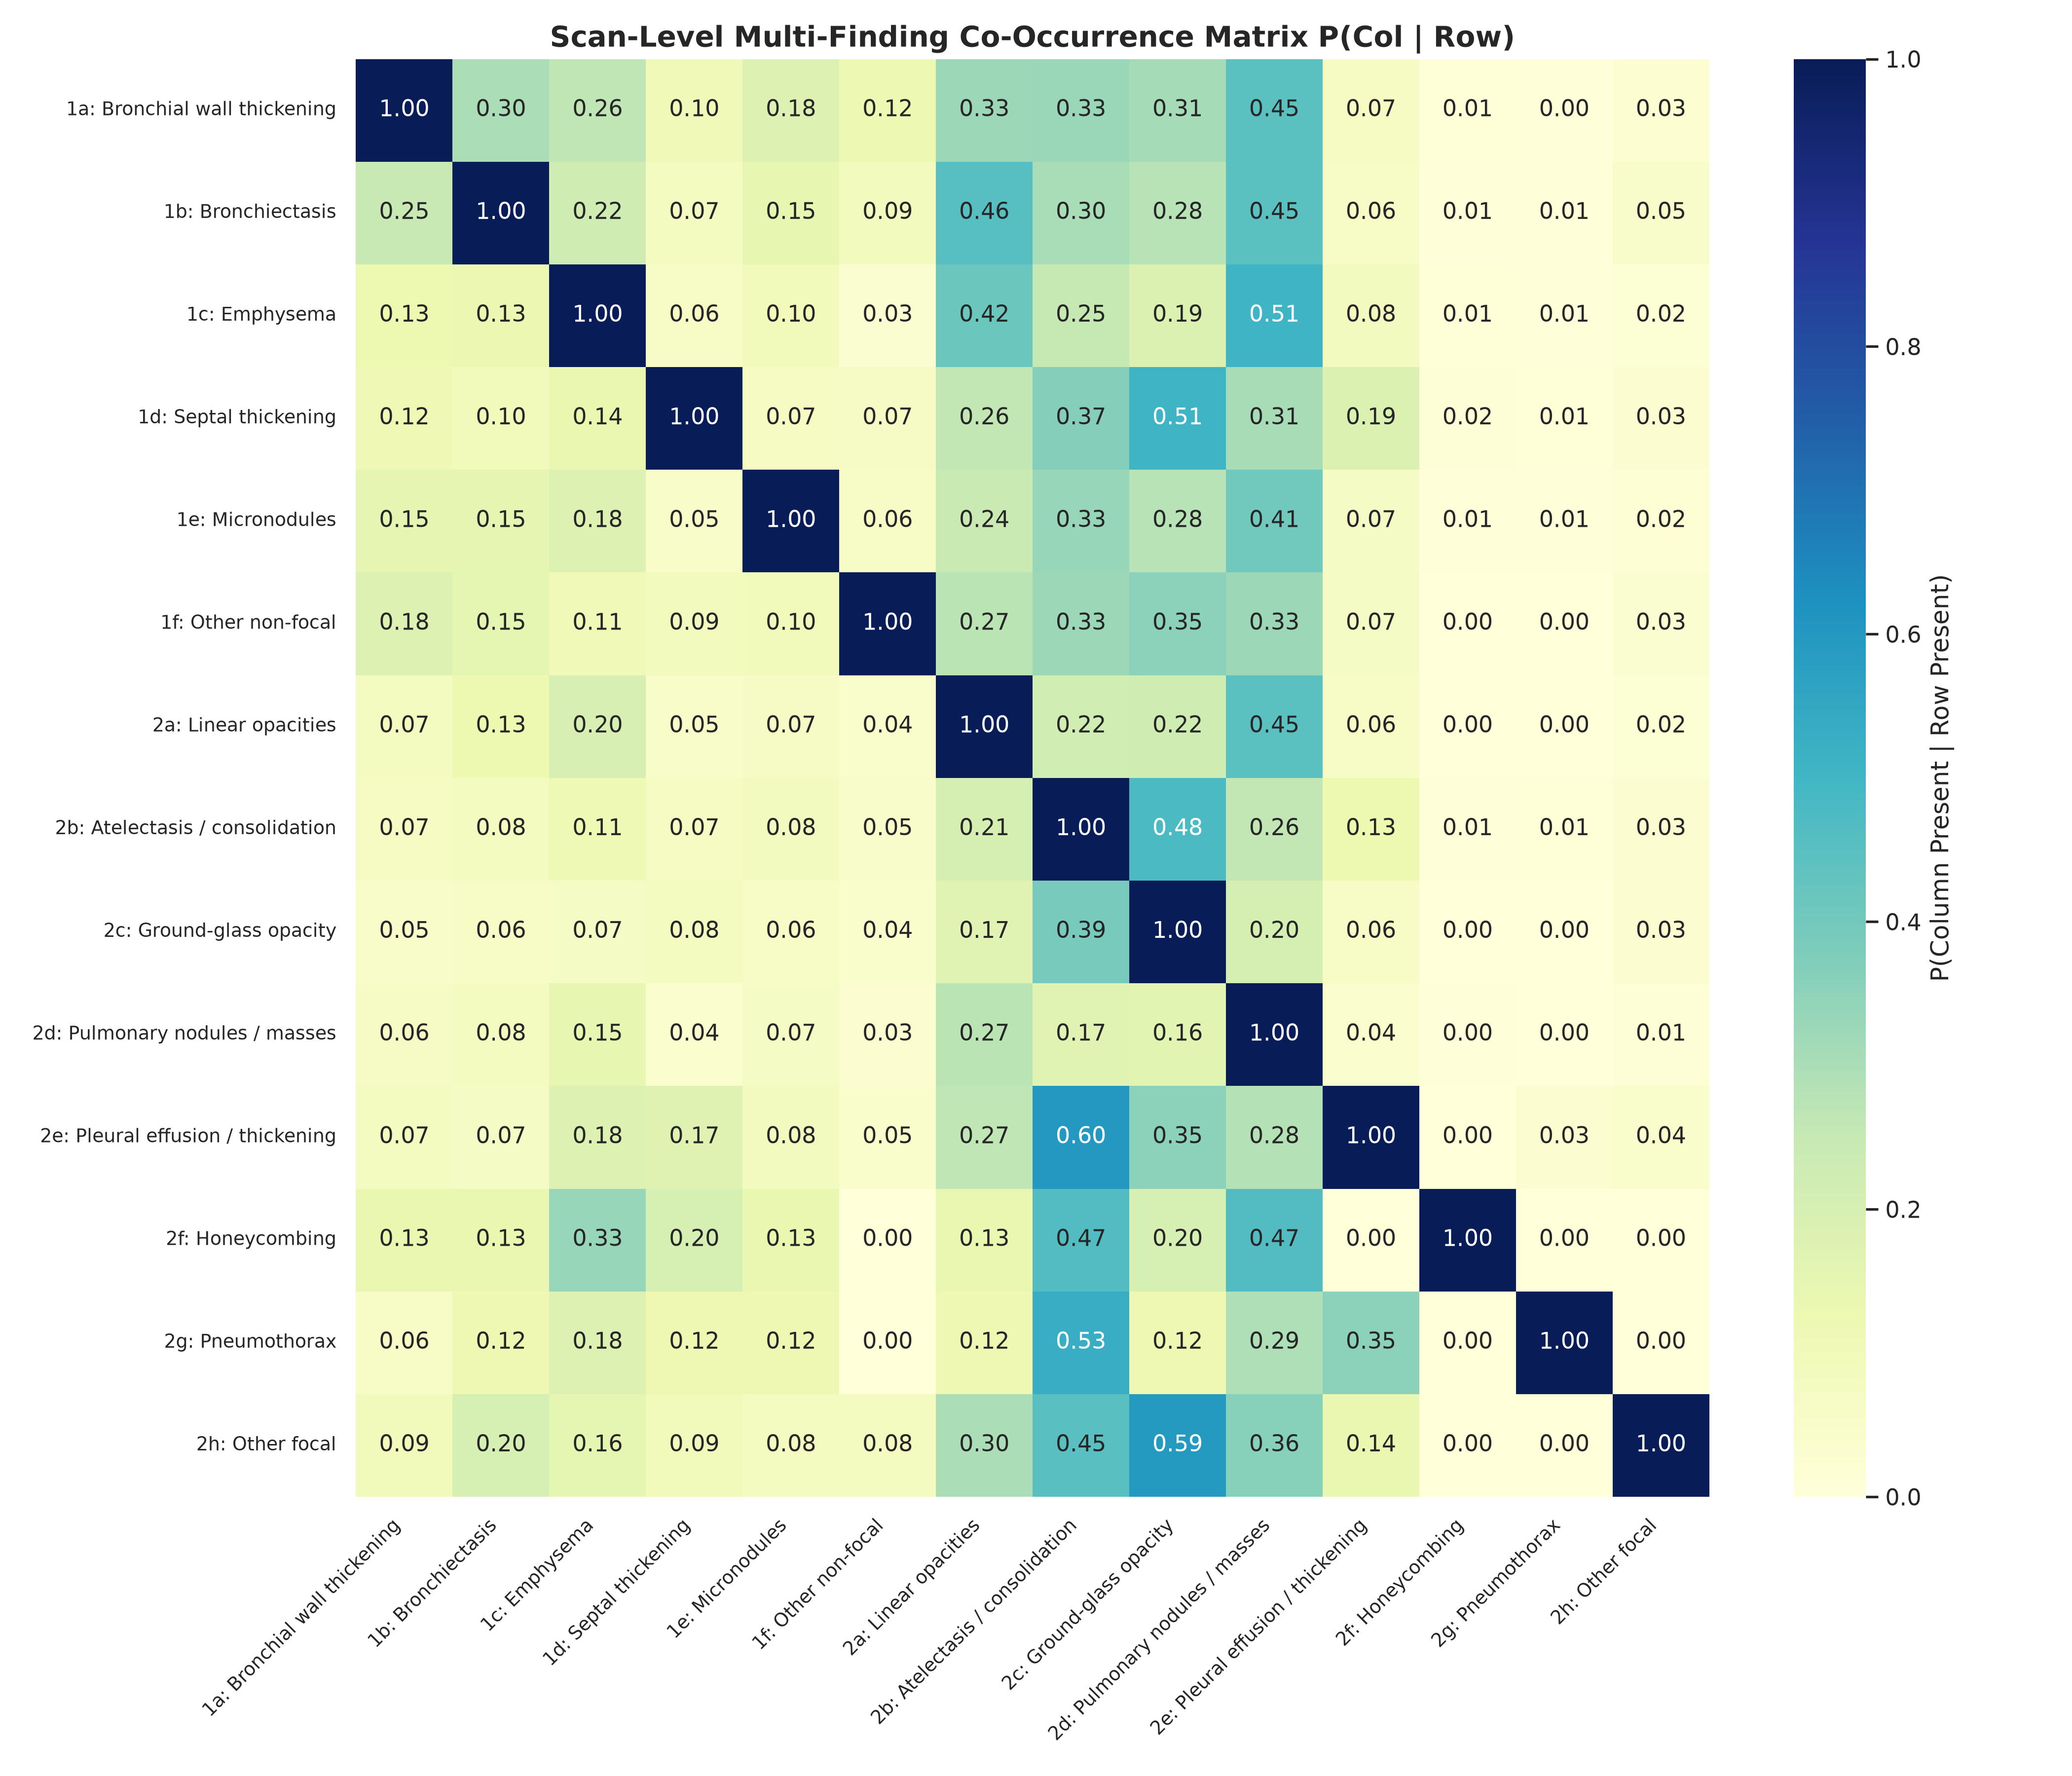
\includegraphics[width=0.75\textwidth, height=0.75\textheight, keepaspectratio]{fig/exp001_cooccurrence_heatmap.png}
    \end{center}

    \note{
        This heatmap shows the 14-by-14 scan-level conditional co-occurrence probability matrix P of category j given category i.

        The heatmap reveals strong clinical dependencies. For example, Pleural effusion co-occurs with Atelectasis in 60 percent of scans, while Honeycombing co-occurs with Atelectasis and Pulmonary nodules in 46.7 percent of scans. Understanding these co-occurrence priors helps model joint pathology detection.
    }
\end{frame}

% ==============================================================================
% SLIDE 8: Table 3 - NLP Syntax Shift
% ==============================================================================
\begin{frame}{Validation Prompt Text Shift (Cases 1--50 vs. 51--200)}
    \centering
    \small
    \setlength{\tabcolsep}{7pt}
    \begin{tabular}{lcccc}
        \toprule
        \textbf{Metric / Parameter} & \makecell{\textbf{Cases 1--50}\\\textbf{(Paper)}} & \makecell{\textbf{Cases 51--200}\\\textbf{(MICCAI)}} & \textbf{Ratio} & \textbf{\% Change} \\
        \midrule
        Total Finding Prompts & 115 & 266 & 2.31x & +131.3\% \\
        Total Word Tokens & 1,263 & 3,193 & 2.53x & +152.8\% \\
        Mean Word Count (words) & 10.98 & 12.00 & 1.09x & +9.3\% \\
        \rowcolor{darkblue!10}
        Max Word Count (words) & 21 & \textbf{35} & \textbf{1.67x} & \textbf{+66.7\%} \\
        Mean Character Length & 70.0 & 80.0 & 1.14x & +14.3\% \\
        \rowcolor{darkblue!10}
        Prompts with Comma Punctuation & 11.30\% & \textbf{23.68\%} & \textbf{2.10x} & \textbf{+12.38\% pt} \\
        Log-Normal TTR (1000 Tokens) & 0.1740 & 0.1651 & 0.95x & -5.11\% \\
        \bottomrule
    \end{tabular}

    \note{
        Here we examine the free-text prompt syntax shift between the paper's original 50 validation cases and the new 150 MICCAI competition cases.

        The new validation prompts show a noticeable increase in syntactic complexity: maximum word length jumps by 66.7 percent up to 35 words, and comma punctuation frequency more than doubles to 23.7 percent.

        Importantly, even with this increased length, subword BPE tokenization expansion remains strictly below 128 tokens across all 8,650 prompts, resulting in zero percent context truncation. Additionally, diagnostic hedging language occurs in only 0.38 percent of prompts.
    }
\end{frame}

% ==============================================================================
% SLIDE 9: Figure 4 - 3D Spatial Probability Density Priors
% ==============================================================================
\begin{frame}{3D Population Spatial Probability Density Priors}
    \begin{center}
        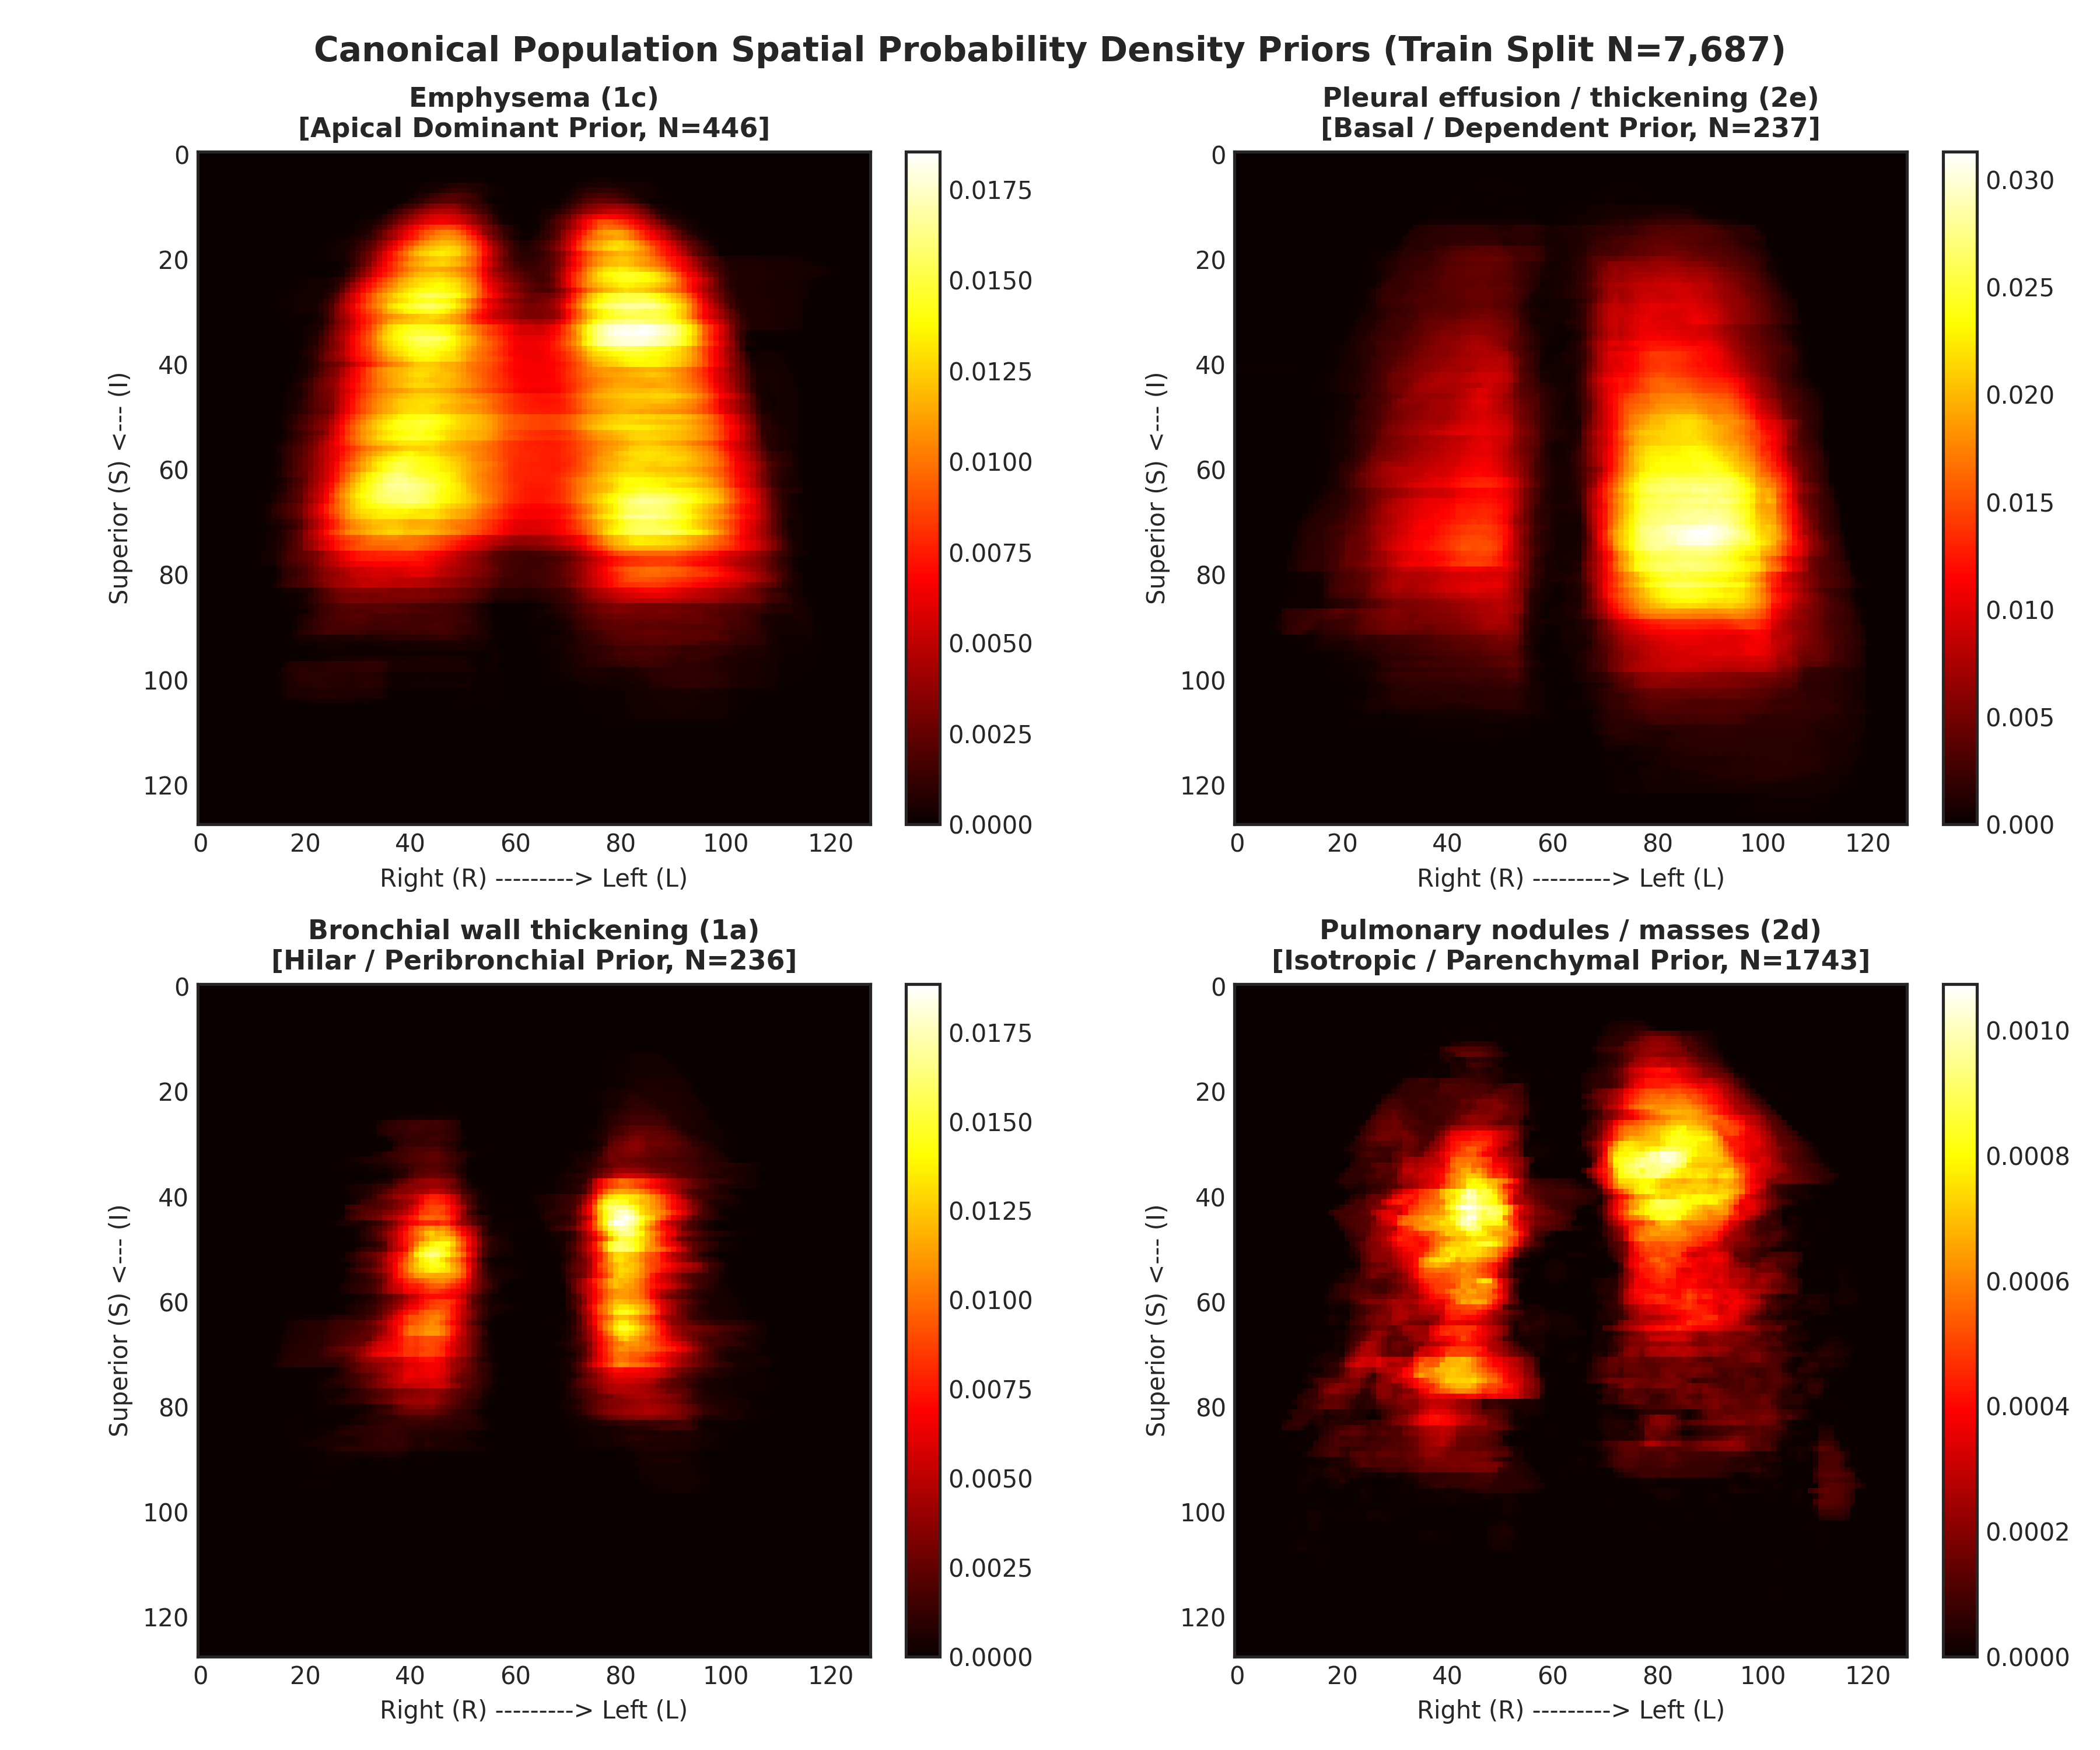
\includegraphics[width=0.82\textwidth, height=0.72\textheight, keepaspectratio]{fig/exp003_population_spatial_priors_4panel.png}
    \end{center}

    \note{
        Here we present coronal projections of population 3D spatial probability density priors across the four spatial taxonomies on a canonical 128-cube RAS grid.

        Notice how the density maps visually confirm our taxonomy rules: Emphysema shows clear upper-zone apical pooling; Pleural effusion and Atelectasis concentrate in gravity-dependent lung bases; Bronchial thickening clusters around central hilar airways; and Nodules exhibit an isotropic parenchymal spread.
    }
\end{frame}

% ==============================================================================
% SLIDE 10: Table 5 - HU Attenuation & Intensity Bounds
% ==============================================================================
\begin{frame}{Hounsfield Unit (HU) Attenuation Profiling}
    \centering
    \scriptsize
    \setlength{\tabcolsep}{7pt}
    \begin{tabular}{clcccc}
        \toprule
        \textbf{Code} & \textbf{Category Name} & \textbf{$N_{\text{masks}}$} & \textbf{Mean HU} & \textbf{Contrast $\Delta \text{HU}$} & \textbf{Rec Window [P5, P95] HU} \\
        \midrule
        \texttt{1a} & Bronchial wall thickening & 239 & -486.35 & -21.98 & [-933.0, +69.0] \\
        \texttt{1b} & Bronchiectasis           & 293 & -477.93 & +1.93  & [-934.0, +86.0] \\
        \texttt{1c} & Emphysema                & 463 & -307.95 & -3.11  & [-992.0, +251.0] \\
        \texttt{1d} & Septal thickening        & 200 & -406.38 & -21.23 & [-1001.0, +121.0] \\
        \texttt{1e} & Micronodules             & 325 & -427.36 & +15.16 & [-998.0, +101.0] \\
        \texttt{1f} & Other non-focal          & 154 & -334.71 & -8.61  & [-987.0, +98.0] \\
        \texttt{2a} & Linear opacities         & 1,189 & -286.55 & +4.68 & [-992.0, +399.0] \\
        \texttt{2b} & Atelectasis / consolid.  & 1,416 & -341.35 & +2.43 & [-995.0, +129.0] \\
        \texttt{2c} & Ground-glass opacity     & 1,567 & -375.11 & -4.51 & [-995.0, +137.0] \\
        \rowcolor{darkblue!10}
        \texttt{2d} & Pulmonary nodules/masses & 1,875 & -427.06 & -49.15 & [-995.0, +194.0] \\
        \texttt{2e} & Pleural effusion/thick.  & 248 & -368.59 & -19.37 & [-1007.0, +135.0] \\
        \texttt{2f} & Honeycombing             & 16  & -420.45 & -18.07 & [-905.0, +83.0] \\
        \texttt{2g} & Pneumothorax             & 19  & -306.85 & -54.68 & [-961.0, +148.0] \\
        \rowcolor{darkblue!10}
        \texttt{2h} & Other focal              & 64  & -156.62 & -16.21 & [-915.0, +201.0] \\
        \bottomrule
    \end{tabular}

    \note{
        This table summarizes Hounsfield Unit attenuation statistics and contrast deltas sampled inside pathology masks versus surrounding parenchyma across 3,192 CT volumes.

        Mean radiodensity ranges from air-filled bronchial thickening at minus 486 HU to soft-tissue opacities like Other Focal at minus 156 HU. Soft-tissue focal lesions show positive contrast deltas against background, whereas nodules and pneumothorax show negative boundary deltas against surrounding parenchyma.

        The last column provides empirical 5th-to-95th percentile HU windowing bounds for category-specific CT intensity preprocessing.
    }
\end{frame}

% ==============================================================================
% SLIDE 11: Table 6 - Morphological Topology & Noise Pruning
% ==============================================================================
\begin{frame}{3D Connected Component Topology \& Pruning}
    \centering
    \scriptsize
    \setlength{\tabcolsep}{3.8pt}
    \begin{tabular}{clccccc>{\bfseries}c}
        \toprule
        \textbf{Code} & \textbf{Category Name} & \textbf{Blobs} & \textbf{Blobs/Find} & \textbf{Sphericity ($S$)} & \textbf{Median Vol ($\text{mm}^3$)} & \textbf{P95 Vol ($\text{mm}^3$)} & Rec Min Size \\
        \midrule
        \texttt{1a} & Bronchial wall thickening & 1,539 & 6.44 & 0.7249 & 90.0 & 88,920.0 & 10 voxels \\
        \texttt{1b} & Bronchiectasis           & 1,007 & 3.44 & 0.6063 & 1,453.0 & 185,597.3 & 10 voxels \\
        \texttt{1c} & Emphysema                & 2,279 & 4.92 & 0.7155 & 578.0 & 193,390.3 & 10 voxels \\
        \texttt{1d} & Septal thickening        & 726 & 3.63 & 0.5434 & 2,844.5 & 197,179.8 & 10 voxels \\
        \texttt{1e} & Micronodules             & 1,210 & 3.72 & 0.7502 & 236.0 & 148,146.1 & 10 voxels \\
        \rowcolor{darkblue!10}
        \texttt{1f} & Other non-focal          & 469 & 3.05 & 0.6177 & 2,664.0 & 305,819.8 & \textbf{47 voxels} \\
        \texttt{2a} & Linear opacities         & 3,248 & 2.73 & 0.6141 & 1,402.0 & 34,399.5 & 10 voxels \\
        \texttt{2b} & Atelectasis / consolid.  & 5,662 & 4.00 & 0.6453 & 943.0 & 126,002.1 & 10 voxels \\
        \texttt{2c} & Ground-glass opacity     & 6,080 & 3.88 & 0.6638 & 1,942.5 & 152,727.0 & 10 voxels \\
        \rowcolor{darkblue!10}
        \texttt{2d} & Pulmonary nodules/masses & 3,836 & 2.05 & \textbf{0.9416} & 192.0 & 3,204.0 & \textbf{15 voxels} \\
        \texttt{2e} & Pleural effusion/thick.  & 749 & 3.02 & 0.5712 & 1,863.0 & 602,883.4 & 10 voxels \\
        \texttt{2f} & Honeycombing             & 55  & 3.44 & 0.6378 & 4,990.0 & 189,603.9 & 10 voxels \\
        \texttt{2g} & Pneumothorax             & 84  & 4.42 & 0.6807 & 42.0 & 261,443.2 & 10 voxels \\
        \texttt{2h} & Other focal              & 194 & 3.03 & 0.6434 & 1,245.0 & 225,928.0 & 10 voxels \\
        \bottomrule
    \end{tabular}

    \note{
        This table details 3D connected-component morphology across 27,138 discrete ground-truth blobs.

        Pulmonary nodules exhibit the highest geometric sphericity at 0.9416, confirming near-spherical focal geometry, whereas Septal thickening and Pleural effusion show low sphericity under 0.58, reflecting planar sheet-like structures.

        The final column specifies empirically derived minimum size thresholds in voxels. For instance, filtering predictions smaller than 15 voxels for Nodules and 47 voxels for Category 1f eliminates small false-positive noise artifacts without losing true recall.
    }
\end{frame}

% ==============================================================================
% SLIDE 12: Ideas para el Challenge
% ==============================================================================
\begin{frame}{Ideas para el Challenge}
    \begin{columns}[c]
        \begin{column}{0.95\textwidth}
            \begin{enumerate}
                \item \textbf{PU Loss Formulation:} PU-SPOCO + Multi-Planar Reconstruction (MPR) consistency loss to handle training label caps ($\le 3$ instances).
                \item \textbf{Category Intensity Windowing:} Preprocess CT volumes using category HU bounds \texttt{[min\_HU, max\_HU]}.
                \item \textbf{Spatial Prior Masking:} Apply 3D RAS spatial probability density priors $P(\mathbf{x}' \in \text{mask} \mid c)$ to bound search space.
                \item \textbf{Component Noise Pruning:} Filter binarized predictions with \texttt{recommended\_min\_size\_voxels} thresholds.
            \end{enumerate}
        \end{column}
    \end{columns}

    \note{
        To conclude, our Phase 1 profiling yields four key ideas for downstream baseline evaluation and fine-tuning:

        First, implement Positive-Unlabeled SPOCO and MPR consistency losses to handle training set label caps.
        Second, apply category-tailored HU intensity windowing bounds rather than naive broad windowing.
        Third, integrate 3D RAS spatial probability priors to constrain candidate search space.
        And fourth, apply component size threshold pruning to remove false-positive noise.
    }
\end{frame}

\end{document}